
%----------------------------------------------------------------------------------------
%	PACKAGES AND OTHER DOCUMENT CONFIGURATIONS
%----------------------------------------------------------------------------------------

\documentclass[10pt, a4paper, twocolumn]{article} % 11pt for all the article

\usepackage{lipsum} % Package to generate dummy text throughout this template

\usepackage{graphicx} % include graphs and images
\usepackage{subfigure} % allow to include multiple graphs under one figure
\usepackage{listings} % include source code

%\usepackage[sc]{mathpazo} % Use the Palatino font
%\usepackage[T1]{fontenc} % Use 8-bit encoding that has 256 glyphs
%\linespread{1.05} % Line spacing - Palatino needs more space between lines
%\usepackage{microtype} % Slightly tweak font spacing for aesthetics

\usepackage[hmarginratio=1:1,left=16mm,right=16mm,top=32mm,bottom=32mm,columnsep=10mm]{geometry} % Document margins
%[left=1in,right=1in,top=0.8in,bottom=0.8in]{geometry

%\usepackage{multicol} % Used for the two-column layout of the document
\usepackage[hang, small,labelfont=bf,up,textfont=it,up]{caption} % Custom captions under/above floats in tables or figures
\usepackage{booktabs} % Horizontal rules in tables
\usepackage{float} % Required for tables and figures in the multi-column environment - they need to be placed in specific locations with the [H] (e.g. \begin{table}[H])
\usepackage{hyperref} % For hyperlinks in the PDF
\usepackage{multirow} % Multiple rows

%\usepackage{lettrine} % The lettrine is the first enlarged letter at the beginning of the text
\usepackage{paralist} % Used for the compactitem environment which makes bullet points with less space between them

%\usepackage{abstract} % Allows abstract customization
%\renewcommand{\abstractnamefont}{\normalfont\bfseries} % Set the "Abstract" text to bold
%\renewcommand{\abstracttextfont}{\normalfont\small\itshape} % Set the abstract itself to small italic text

%\usepackage{titlesec} % Allows customization of titles
%\renewcommand\thesection{\Roman{section}} % Roman numerals for the sections
%\renewcommand\thesubsection{\Roman{subsection}} % Roman numerals for subsections
%\titleformat{\section}[block]{\large\scshape\centering}{\thesection.}{1em}{} % Change the look of the section titles
%\titleformat{\subsection}[block]{\large}{\thesubsection.}{1em}{} % Change the look of the section titles

%\usepackage{fancyhdr} % Headers and footers
%\pagestyle{fancy} % All pages have headers and footers
%\fancyhead{} % Blank out the default header
%\fancyfoot{} % Blank out the default footer
%\fancyhead[C]{Running title $\bullet$ November 2012 $\bullet$ Vol. XXI, No. 1} % Custom header text
%\fancyfoot[RO,LE]{\thepage} % Custom footer text

\usepackage{amssymb} % for math symbols (e.g.  \Join)


%----------------------------------------------------------------------------------------
%	TITLE SECTION
%----------------------------------------------------------------------------------------

\title{\vspace{-15mm}\fontsize{18pt}{10pt}\selectfont\textbf{DaSci: Large Scale Textual Data Visualization}} % Article title

\author{
  \textbf{Julien Ribon}\\
  \textbf{EPFL}
  \and
  \textbf{Michele Catasta}\\
  \textbf{EPFL}
  \and
  \textbf{Karl Aberer}\\
  \textbf{EPFL}
  \and
  \href{mailto:julien.ribon@epfl.ch}{\textbf{\{julien.ribon, michele.catasta, karl.aberer\}@epfl.ch}}
}
\date{}


%\author{
%\large
%\textsc{Julien Ribon} \\ %\thanks{A thank you or further information}\\[2mm] % Your name
%\normalsize University of California \\ % Your institution
%\normalsize \href{mailto:julien.ribon@epfl.com}{\{ julien.ribon, manos.karpathiotakis, danica.porobic, anastasia.ailamaki \}@epfl.com} % Your email address
%\vspace{-5mm}
%}
%\date{}

%----------------------------------------------------------------------------------------

\begin{document}

\maketitle % Insert title

%\thispagestyle{fancy} % All pages have headers and footers

%----------------------------------------------------------------------------------------
%	ABSTRACT
%----------------------------------------------------------------------------------------

%\begin{multicols}{2} % Two-column layout throughout the main article text

\begin{abstract}

The amount of unstructured data is increasing drastically and is today the most common form of data format, overtaking structured data such as relational databases and semi-structured files.
Sate-of-the-art machine learning algorithms can be used to extract features and build general-purpose representation of meaning from unstructured data. This meaning can then be visualized in a reduced dimensional space.
On the other hand, significant progress has been made in the exploration and visualization of large multi-dimensional databases.
But, so far, little work has been devoted to bridge technological advancements made in relational databases with textual information extraction.
In this paper, we present DaSci, a system for exploring unstructured datasets, which extracts features out of raw text, maps these features into a general-purpose data model, and provides an interface based on a relation-like, tabular level of abstraction to visualize multi-dimensional data.
Retrieving data, extracting information and gaining insights is achieved in real time, while visual representations can rapidly be constructed out of raw textual data. \\

Keywords:
\textit{data analysis, multidimensional data modeling, data visualization, information extraction.}


\end{abstract}

%----------------------------------------------------------------------------------------
%	ARTICLE CONTENTS
%----------------------------------------------------------------------------------------


\section{Introduction}
\label{section:introduction}

As the amount of data is doubling every two years, many organizations struggle to analyze and make use of their datasets. Not only is the data continuously increasing in size but also in terms of source variety. The major part of that data is unstructured, i.e. in form of plain-text documents, and therefore not directly exploitable with state-of-the-art data management systems.
OLAP systems offers rigid mapping-based ETL for converting and formatting raw datasets. This process usually takes more than 80\% of the whole analysis process \cite{etl}. Moreover, business analysts and data scientists usually rely on IT experts to prepare and access their data, which often requires days or sometimes even months before analysts can start working on their data. Even with a specific business model in mind, data analysts and scientists do not necessarily know about the insights and categories they are looking for, thus, making the whole analysis process even more cumbersome. 
Successful analysis relies upon accurate, well-structured data that has been massaged for specific needs of the task at hand. 
To drive innovation, it is therefore crucial for companies to be able to quickly and intuitively extract knowledge from their underlying data sources. % and added value.

Our line of work is at a cornerstone between three major research areas, namely multidimensional data management, machine learning, and data visualization.  
First, we design an adaptive data model, called \textit{data grid}, that dynamically adjusts its schema as new datasets are joined together and evolves gracefully as new data dimensions and categories are discovered.
A data grid is at a sweet spot between the key-value processing paradigm \cite{map-reduce} in that it seamlessly scale up in terms of both quantity and diversity of data, and multi-dimensional relational databases in that business users access their data in tabular format using a spreadsheet-like interface (similar to pivot tables).
Second, machine learning capabilities are used to span a whole multi-dimensional vector space out of a corpus of documents and then reduce the number of dimensions to extract meaningful features.
Once identified, those feature are transformed into a columnar representation that is much easier to interpret and visualize.  
The long-term idea is to create a symbiosis between human analysts and the machine, so that users can help the machine to extract useful information. 
Finally, we design an interactive processing and visualization environment that assists analysts through the whole data preparation process (including data discovery, structuring, cleaning, enrichment, and validation) and allows them to automatically derive knowledge from their assets by providing intuitive visual representations of the transformed data.

In addition to the adaptive data model that deals with the variety of data, we design a system architecture that copes with the volume of data. DaSci follows three key principles that shape the overall system architecture: fine-grained caching, decoupled communication and on-demand sampling. Together, these principles allow DaSci to handle large datasets on the fly, without requiring any blocking ETL operations.
In order to illustrate how data analysts and scientists can benefit from DaSci, we implement a prototype based on Spark \cite{spark, rdd}, which empowers end-users with the ability to quickly explore, transform and visualize large amount of both structured and unstructured data.

To investigate the performance of DaSci, we run two types of experiments. The first experiment compares DaSci's response time with in-production data wrangling systems. Retrieving data and extracting information from raw textual data is achieved in human-acceptable delay times, i.e no more than few seconds.
In the second experiment, we illustrate how database processing techniques can be used in symbiosis with machine learning algorithms to structure raw textual data. To this extent, we implement three algorithms to derive vector features (TF-IDF, Word2Vec, and LDA) and apply dimension reduction for interpretation and visualization purposes.

The rest of this report is organized as follow. In section \ref{section:related-work}, we present earlier work done in large multi-dimensional relational databases, as well as NLP and visualization systems. In section \ref{section:approach}, we introduce the general-purpose data model, as well as the core concepts on which DaSci is based. In section \ref{section:system}, we describe DaSci's primary components and give a brief description about its caching, communication and sampling infrastructures. Section \ref{section:experiments} presents experimental results and show the performance of DaSci compared to other data-wrangling systems. Finally, we suggest possible further enhancements in section \ref{section:future-work} and end this paper with some concluding remarks in section \ref{section:conclusion}.


\section{Related Work}
\label{section:related-work}

There are already several software products that can be used for data wrangling, such as Trifacta Wrangler \cite{wrangler, trifacta} and Idibon \cite{muck, mitext}, which offer data transformations and interactive visualization.
Moreover, in recent years, novel natural language processing applications have emerged. Among them, NLTK is a well-known platform to work with human language data that provides easy-to-use interfaces, lexical resources, along with a suite of text processing libraries for classification, tokenization, stemming, tagging, parsing, and semantic reasoning \cite{nltk}.
Stanford CoreNLP \cite{core-nlp} also provides a set of natural language analysis tools that can give the base forms of words, their parts of speech, recognize entites, or mark up the structure of sentences. 
However, so far, little work has been devoted to wrangle raw text data using natural language processing tools. In this work, we study how data wrangling and NLP techniques can be combined with large-scale machine learning capabilities.

In the data visualization literature, most recent works have been devoted to exploring large relational databases. 
Polaris \cite{polaris} is a system for querying, analyzing, and visualizing multidimensional relational databases, which has been commercialized as Tableau. In that work, C. Stolte et al. developed a dense graphical representation that extends the well-known pivot table interface. We draw inspiration from their work to design the \textit{pivot grid} interface, presented in section \ref{subsection:pivot-grid}.
Other application software focus on automatic presentation over user experience \cite{show-me} and database queries for efficient visualization\cite{seedb}.
However, these software are limited to relational database systems and do not deal with unstructured datasets in any way. In this paper, we develop a software architecture that leverages advancements made in relational database visualization and apply these techniques to textual information extraction and exploration.
Furthermore, significant work has also be done in multi-dimensional data sampling and pre-fetching to offers intuitive and interactive visualization interface to end-users.
L. Lins et al. introduce a new data structure called \textit{nanocube} \cite{nanocubes}, i.e. a data cube that fits in a laptop's main memory, that is used for real-time exploration of large multidimensional spatio-temporal datasets. Nanocubes use a two-layer prediction engine together with cache allocation strategies to deliver concise data summaries.
ForCache \cite{data-tiles} is a general-purpose tool for exploratory browsing of large datasets based on a client-server architecture and following a detail-on-demand browsing paradigm.
In this work, we design a similar client-server architecture and investigate how our system can benefit from fine-grain caching and on-demand sampling strategies to construct multidimensional hypercubes. 


\section{Approach}
\label{section:approach}

In this section, we explain the motivations and principles of our data model and lay down the foundation of the DaSci system.


\subsection{The Data Grid Model}
\label{subsection:data-grid}

The Data Grid model is a relation-like, tabular level of abstraction, whose goal is to bridge the recent NoSQL technologies made in the last decade together with the relational model, while giving to data analysts and scientists control and knowledge over their data. 

The datagrid is based on the concept of dataframe, a distributed collection of data organized into named columns. A DataFrame is conceptually equivalent to a table in a relational database, but with richer in-memory optimizations under the hood\cite{spark}. DataFrames can be constructed from a wide array of sources such as external database tables, as well as structured data files (e.g. CSV, JSON, and XML).
Once created, a DataFrame can be manipulated using the various domain-specific-language (DSL) functions.
The datagrid is an extension of this concept in the sense that a datagrid represents several potentially-related DataFrames.

The main idea behind the datagrid paradigm is that there is only one large data collection rather than several independent, disjoint datasets. This means that all the data is virtually represented by a single, unbound collection.
Hence, a datagrid can represent an entire relational database or even several databases, where all tables are joined together in one large but very sparse denormalized table.
Furthermore, several independent structured files can easily be combined together into the same datagrid, especially if these files are sharing a common group of fields or columns.

In order to seamlessly combine several datasets based on their inferred schema, we define and implement a new joining algorithm, called \textit{u-join}.
A \textit{u-join} is similar to a full outer join except that non-matching tuples are still added to the resulting data table. 
Moreover, when there is no common columns to join the datasets, all columns from both datasets are first combined together before adding their respective tuples independently. In the later case, this is equivalent to compute the "union all" operator between two tables sharing the same columns, except that here datasets do not necessarily share any common columns.

We illustrate the \textit{u-join} algorithm with the following example. Assuming we have two datasets $D_F$ and $D_G$, which have schema $\{a,b,c\}$ and $\{b,c,d,e\}$ respectively. We can see dataset $D_G$ as representing the datagrid and $D_F$ being an independent DataFrame that must be incorporated within the datagrid.
For simplicity, we assume that all column are of type \textit{string}.     
A \textit{u-join} is then equivalent of executing the following query after adding the missing columns to the original datagrid:

\begin{lstlisting}[numbers=none]
    SELECT a, b, e, 
     COALESCE(DG.b,DF.b) as b, 
     COALESCE(DG.c,DF.c) as c
    FROM DG
    FULL OUTER JOIN DF ON 1=1
     AND DG.b = DF.b
     AND DG.c = DF.c
\end{lstlisting}

Integrating dataset $D_F$ into $D_G$ using the \textit{u-join} therefore results in a new datagrid $D_G'$ with schema $\{a,b,c,d,e\}$.

Now, assuming that we have another dataset $D_H$ with columns $\{x,y\}$ and that each dataset contains exactly two tuples, then a possible resulting datagrid $D_G''$ with schema $\{a,b,c,d,e,f,g\}$ is shown in table \ref{table:datagrid}. In this example, only one tuple between $D_F$ and $D_G$ was joint, whereas no tuple could be joint between $D_H$ and other datasets since they share no common column.

\begin{table}[H]
	\centering
	\begin{tabular}{lllllll}
	\toprule
	%\multicolumn{2}{c}{Name} \\
	%\cmidrule(r){1-2}
	$a$ & $b$ & $c$ & $d$ & $e$ & $f$ & $g$ \\
	\midrule
	$a_1$ & $b_1$ & $c_1$ & $null$ & $null$ & $null$ & $null$ \\
	$a_2$ & $b_2$ & $c_2$ & $d_2$ &  $e_2$  & $null$ & $null$ \\
	$null$ & $b_3$ & $c_3$ & $d_3$ &  $e_3$  & $null$ & $null$ \\
	$null$ & $null$ & $null$ & $null$ &  $null$  & $f_4$ & $g_4$ \\
	$null$ & $null$ & $null$ & $null$ &  $null$  & $f_5$ & $g_5$ \\
	\bottomrule
	\end{tabular}
	\caption{Resulting datagrid when $D_f$, $D_g$ and $D_h$ are joined using the u-join algorithm.}
	\label{table:datagrid}
\end{table}

%Formally, the \textit{u-join} operator is defined as follow: \\
%$D_F \Join_u D_G = \{x \cup y | x \in D_F \wedge y \in D_F  \wedge\ f(x \cup y) \},$ \\
%$f(x,y) = \{x \cup y | \forall x_i \in x, y_j \in x, x_i = y_j \}$ \\

As we will see in section \ref{subsection:pivot-grid}, one outcome of using such data paradigm is the ability to scale the retrieval of high-dimensional datasets.
 

\begin{figure}
	\centering
	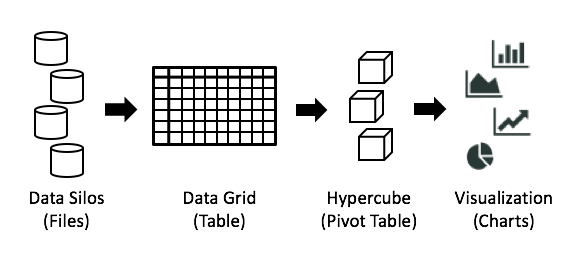
\includegraphics[scale=0.4]{images/concepts.png}
	\caption{Core Concepts}
	\label{figure:concepts}
\end{figure}


\subsection{From Text to Structured Data}
\label{subsection:text-data}

The amount of natural language text that is available in electronic form is increasing drastically and is today the most common form of data format.
However, the complexity of natural language can make it very difficult to access the information contained in raw text. Also, the state of the art in NLP (Natural Language Processing) is still a long way from being able to build general-purpose representation of meaning from unrestricted text. However, if we focus our efforts on a limited set of questions by deciding in advance to look only for very specific kind of information (e.g. entity recognition, keyword extraction, topic modeling, etc.), then it is possible to make significant progress.
It is therefore essential to (i) convert natural language sentences of unstructured text into structured data, and (ii) identify which methods and corpora are appropriated to obtain useful information from text.
Figure \ref{figure:information-extraction} show an example of information extraction pipeline that transforms raw text into entities and relationships \cite{nltk-book}. 


In order to extract knowledge automatically from a given corpus, we consider the vector space model that represents text documents as vectors in a multi-dimensional space.
It is important to note that the multi-dimensional vector space is of different nature than the multi-dimensional space spanned by a hypercube, as described in section \ref{subsection:pivot-grid}.
In fact, there is an impedance mismatch between the hypercube and vector space, as both can represent the data in a multi-dimensional space, yet with incompatible dimensions.
To make these two multi-dimensional space compatible, the idea is to map one space into the other. Here, we focus on mapping the vector space (of extracted features) into the datagrid's column space, where each vector value is converted into a column value and mapped to a hypercube dimension (eventually spanning new dimensions). This is equivalent to applying a linear map that transforms the whole vector space into column space.
Every vector representing a certain document is thus transformed into a sparse row in the DataGrid, where every non-null column represents a dimension from the original vector space.

Formally, this linear map can be described as follow.
Function $f : V \mapsto D$ is a linear map from the vector space $V$ to the multi-dimensional space spanned by the datagrid $D$, where for any two feature vectors $x$ and $y$ in $V$ and any weight (scalar) $\alpha$ in field $K$, additivity and homogeneity are satisfied, i.e. $f(x+y)=f(x)+f(y)$ and $f(\alpha * x) = \alpha * f(x)$, respectively.
Function $f$ therefore transforms each dimension from the vector space $V$ either by mapping the original dimension into an existing datagrid's dimension or by spanning a new one if necessary.

%\begin{compactitem}
%\item{Additivity}: $f(x+y)=f(x)+f(y)$
%\item{Homogeneity}: $f(\alpha * x) = \alpha * f(x)$ \\
%\end{compactitem}



Converting the vector space into the datagrid space is essential as this will allows us to build hypercubes in order to summarize and, later, visualize data, as illustrated in the following section.

%In fact the growth ratio between structured  (block) and unstructured (file) data is dramatically different, as shown in Figure \ref{figure:...} \cite{idc}: in 2014, unstructured data represented more than 85\% while structured data accounted for only 15\%.
%Now that our d that can represent a potentially-infinite amount of structured data, we need a mechanism to summarize this unbounded data collection.



\subsection{NoLAP Hypercube}
\label{subsection:pivot-grid}

The next important concept is the NoLAP (Not only OLAP) hypercube \cite{cell} used to summarize large datasets. In DaSci, we present this hypercube abstraction to end-users through a so-called \textit{pivotgrid}.

OLAP targets multi-dimensional data that is represented as a data cube and stored in either star or snowflake schema inside a relational data warehouse. Spreadsheets and business intelligence software then visualize the underlying data cubes in a more business-friendly way by using a data-summarization mechanism called pivot table. As such, pivot table is an abstraction of the more complete and complex OLAP functionality.

OLAP usually comes in two major flavours: ROLAP (relational databases) and MOLAP (hypercube in memory). However, in both cases, the shape of your hypercubes must be defined in advance into a rigid schema. And neither of these OLAP techniques do scale well with the number of dimensions, as the number of tables necessary to build the data cubes explodes. This phenomena is known as the curse of dimensionality.

Following the NoSQL paradigm, however, NoLAP do not require hypercubes to be prepared or stores in advance. 
It is therefore possible to build any arbitrary hypercube at runtime and to retrieve any number of dimensions on-the-fly in real time.
NoLAP has therefore the advantage of storing virtually all dimensions into a single malleable table (with virtually no performance penalty), rather than spreading dimensions over several rigid tables.

In short, a pivotgrid is to the datagrid model what a hypercube is to OLAP (Online Analytical Processing), or (in a higher level of abstraction) what pivot table is to spreadsheets and business intelligence software. 
In the context of our datagrid paradigm described in section \ref{subsection:data-grid}, a pivotgrid is a consolidated representation of a high-dimensional hypercube created from a subset of all datagrid's dimensions.
If we combine this approach with the linear transformation described in section \ref{subsection:text-data}, it is then possible to leverage OLAP's capabilities over raw textual data.

Building a whole OLAP cube usually requires a full IT expertise that often take months to complete. Furthermore, from an analyst's point of view, a hypercube still displays the data in a very raw structure. 
The pivotgrid therefore offers to end-users a tabular abstraction of the underlying hypercube by flattening the data into two-dimensional space, like a pivot table.
This allows end-users to interact with multidimensional through a clear and comprehensible interface without requiring any IT intervention. 

The next step in data analysis is then to visualize the underlying hypercube, which can easily be achieved by building a pivot graph on top of the pivotgrid abstraction.



\section{The DaSci System}
\label{section:system}

This section presents the structure, goals and boundaries of our system. 
In particular, the DaSci system is based on the following key concepts: \\

\begin{compactitem}
\item{\textit{Data Silos}}: Heterogeneous data sources can be connected to DaSci. The imported data is then distributed and replicated across a cluster, where it can efficiently be retrieved and summarized using the MapReduce processing paradigm \cite{map-reduce}. \\
\item{\textit{Data Grid}}: The datagrid model exposes denormalized data silos as a single tabular abstraction to end-users. Schema are automatically inferred and adapted to conceive domain-specific taxonomies. Further features can be extracted from textual columns (e.g. representing a corpus of documents) and transposed into the datagrid's column space. This is especially useful for indexing and deriving more precise information out of unstructured data. \\
\item{\textit{Data Hypercubes}}: DaSci handle highly dimensional data and exposes to end-users the data cube abstraction via a familiar spreadsheet-like interface, i.e. the pivotgrid. Using the pivotgrid, end-data scientists and analysts can easily slice, dice, and aggregate datagrid's dimensions. \\
\item{\textit{Data Visualization}}: After massaging the underlying data through the datagrid and preparing a concise summary out of the multi-dimensional hypercube, insights and knowledge can then be obtained by visualizing the data into clear-cut graphical representations. \\
\end{compactitem}

These concepts are illustrated in figure \ref{figure:concepts} as a 4-step pipeline going from data silos up to data visualization. In the remainder of this section, we explain in more details how the workflow between these concepts takes place and what system component is responsible for each stage.



\subsection{System Architecture}


\begin{figure}
	\centering
	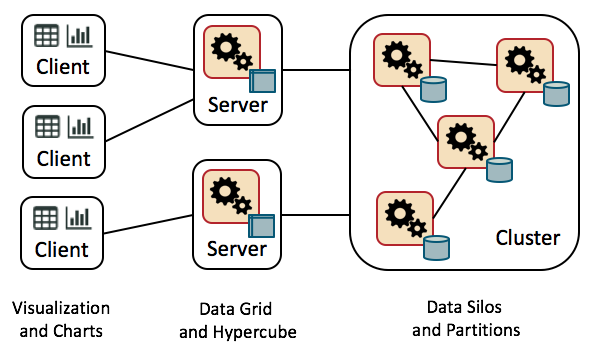
\includegraphics[scale=0.35]{images/system.png}
	\caption{DaSci's System Components}
	\label{figure:system}
\end{figure}


The DaSci system is composed of three major parts: \textit{client}, \textit{server} and \textit{cluster}.
Figure \ref{figure:system} illustrates these different system components and shows how they interact with each other. 

The cluster is responsible for connecting, storing and retrieving large heterogeneous datasets from several independent resources; we call these datasets \textit{data silos}. 
The following code represents a connection to a specific data silo:

%or \tiny \small or \footnotesize etc.
\begin{lstlisting}[numbers=none,basicstyle=\small] 
  {"id":     1,
   "count":  5171075,
   "type":   "file",
   "format": "xml",
   "size":   "49 GB",
   "name":   "enwiki-articles.xml",
   "path":   "hdfs://localhost:9000/data"}
\end{lstlisting}


Statistics are lazily derived from new data sources once they are connected to DaSci. In particular, counting the number of items in a given data source is important, as this information can be used to improve data partitioning and sampling, which later ensure efficient data retrieval.
Also, another important goal of the cluster is to abstract several data silos into a single datagrid (a relation-like, tabular level of abstraction presented in section \ref{subsection:data-grid}), and to carry out large transformations over the whole set of data silos.

Besides accepting client connections and handling client requests, the server aims at providing fast data sampeling and summarization from the much larger and diverse datasets. The server is indeed a middleware that is responsible to handle the multi-dimensional hypercube and to build the pivotgrid out of a sampled datagrid. It is also the role of the server to hide details and complexity from the back-end cluster.

The client, i.e. the front-end component, is mainly responsible for interacting with end-users and offering data visualization capabilities. In addition, the goal of the client is also provide disconnected operations, as well as both synchronous and asynchronous communication with the server and cluster respectively.
The key idea is to offer an interactive environment for data analysts, so that they have the impression to work on the complete dataset while still obtaining real-time responses.


\subsection{Caching}

\begin{figure}
	\centering
	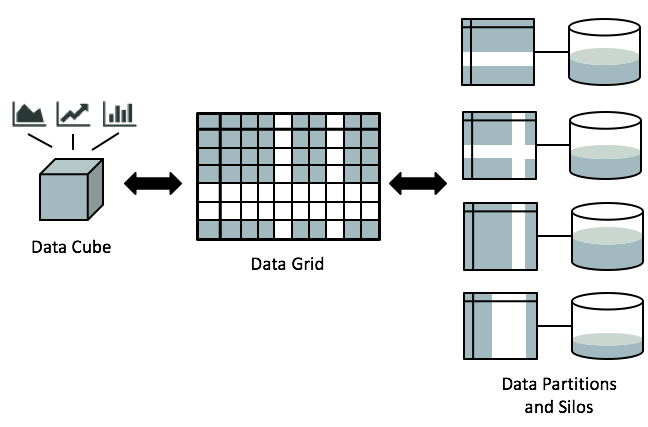
\includegraphics[scale=0.3]{images/caching.png}
	\caption{Caching Infrastructure}
	\label{figure:caching}
\end{figure}

It is not possible to issue queries directly on a complete, very large dataset and to obtain human-acceptable response time. Yet we would like to provide end-users with seamless interactions, real-time operations and transformations, while giving the impression that operations are performed on whole data silos. 
To this extent, we design an infrastructure based on (i) fine-grained caching, (ii) decoupled communication and (iii) on-demand re-sampling.
In this section, we start by explaining how we implement the caching infrastructure in DaSci.
Communication and sampling mechanisms are explained in section \ref{subsection:communication}.

Figure \ref{figure:caching} represents how DaSci enables fine-grained caching through every layer of the pipeline.
When possible, DaSci caches the entire pivotgrid, i.e. graphical data is cached at the client side, while the hypercube is cached at the server side.
As explain in section \ref{subsection:pivot-grid}, the pivotgrid is based on a subset of the datagrid's columns and rows.
Therefore, DaSci only keeps those columns and rows in the server cache.
If enough free space is available however the entire datagrid is cached at the server.

Under the hood, the datagrid is usually divided into several data partitions stored at different locations and often spanning several data silos. In these cases, it is important that the appropriate rows and columns are also cached in their respective nodes in the cluster. 
Cluster caches are especially useful when DaSci needs to re-sample the datagrid, as explained in the next section.

Another aspect that must be considered when dealing with large datasets is the way data is organized across partitions. We decide not to organize the cluster in any logical way and let Spark handle the partitioning. However, in the server cache, each sampled datagrid is organized into a single partition. This has the advantage to alleviate the burden of issuing parallel processing tasks when dealing with small datasets.


\subsection{Communication and Sampling}
\label{subsection:communication}


\begin{figure}
	\centering
	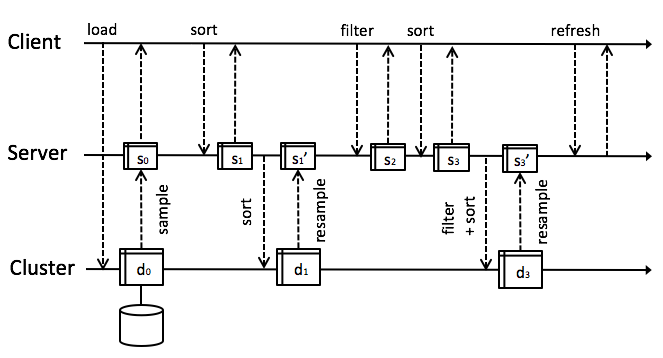
\includegraphics[scale=0.35]{images/communication.png}
	\caption{Sampling  and Communication Mechanisms}
	\label{figure:communication}
\end{figure}

When dealing with very large datasets, fine-grained caching is often not enough to enable real-time responses while obtaining precise summaries and statistics.
Even if only a small portion of the data is subject to caching, that data may still be to large to visualize or even to fit in memory without further filtering and dimension reduction.
Fortunately, it is not necessary at all to cache the whole data, as data analysts are only interested in (and can only study) a small portion of data at a time.
Therefore, it is enough to only deliver a smaller subset of the data of interest by sampling the complete, much larger dataset.

One possible way to implement data sampling, is to sample the whole dataset after each user operation. This approach does not scale well however, as recomputing a new sample from the whole dataset after each transformation can be very expensive. 
A better approach is therefore to re-sample only when absolutely necessary, i.e. when the original sample does no longer represent the population well.
This happens for instance when data transformation has to be done on the whole dataset (e.g. sorting) or when the current sample become to small due to filtering with low selectivity.
It is therefore essential to provide a fast re-sampling mechanism, so that the sample almost always estimate characteristics of the whole population.

Figure \ref{figure:communication} illustrates the sampling and communication mechanisms in DaSci.
First of all, it is important to note that communication between system components are always synchronous. Nevertheless, servers form a middle layer that aims at decoupling client from cluster processing, giving a asynchronous-like communication mechanism between clients and the cluster.

The client sends data transformations one-by-one to the server, which in turn applies each transformation on the appropriate datagrid and stores the transformation in a pending list.
Next, based on the last data transformation and the resulting datagrid, the server decides whether re-sampling is necessary. If so, the server sends all pending transformations to the cluster and asks the cluster to re-sample the datagrid. The server will not re-ask the cluster before receiving an update.

When a client issues a "load" request for the first time on a dataset, the synchronous request is forwarded to the cluster, which caches the data in all participating nodes, samples the dataset, and sends the updated data.
Sampling in DaSci is done randomly. So, in order to ensure that the same subset is returned after each re-sampling, we use a fixed seed value for all samples.
Next, every time a transformation (such as sorting) must be executed on the entire dataset, the synchronous call from the client is immediately answered by the server that, in turn, sends an equivalent request to the cluster. Once the transformation has been applied to the whole dataset, the cluster sends a new sample to the server that then updates the datagrid accordingly.
The request between server and cluster is completely transparent to the client. This means that the client can continue to work independently (with the server) while larger data transformations are issued to the cluster. Updates only become visible to clients once they issue a new transformation request.


\subsection{Data Transformations}

The ability to rapidly display the datagrid and visualize the pivotgrid is vital but not sufficient to ensure interactive exploration.
Additional interactivity such as display manipulation is needed. Analysts must be able to transform the underlying data in order to uncover meaningful relationships and extract useful information. Analysts must also be able to form ad-hoc grouping and partitioning that reflects the newly uncovered infromation \cite{polaris}.
DaSci possesses several types of transformations to support data analysis: feature extraction, sorting and filtering, as well as undo and redo operations.
  

\begin{figure}
	\centering
	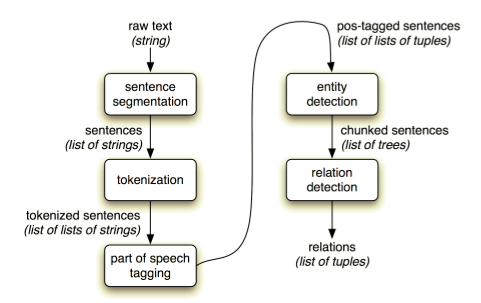
\includegraphics[scale=0.5]{images/information-extraction.png}
	\caption{Example of Pipeline for Entity-Relationship Recognition \cite{nltk-book}}
	\label{figure:information-extraction}
\end{figure}
  
  
\subsubsection*{Deriving Features}

While analyzing data, one of the most important interaction is the ability to derive additional features from the original, potentially-unstructured data. In our system, the main feature derivation mechanism is the extraction of information out of raw textual data.
But DaSci also provides other mechanisms such as grouping and splitting.
%Adding derived features on the fly is necessary as part of the exploration and analysis process.

\textit{Feature extraction} allows to transform arbitrary text into numerical features usable for machine learning. 
In DaSci, all feature extraction techniques are implemented as \textit{pipelines}, where each transformation takes as input an original datagrid and outputs a transformed datagrid that in turn becomes the input for the next stage.
We implement three algorithms for feature extraction: TF-IDF, Word2Vec and LDA.
Figure \ref{figure:information-extraction} shows a simple pipeline for entity recognition and relationship detection, where sentence segmentation, tokenization, and POS-tagging are distinct pre-processing stages.

\textit{Labeling} allows to mark a subset of data and augment each data item with some sort of meaningful tag, class or label that is somehow informative or desirable to know. Labeling is one of the simplest way of adding meaning to the underlying dataset and is especially useful for training supervised learning algorithms.

\textit{Grouping} allows to quickly group together similar column values and apply simple aggregation functions to other dimensions.
These arbitrary grouping and aggregation operations are powerful because they allow analysts to add their own domain knowledge and adapt their groupings as the exploration uncovers additional patterns.

\textit{Splitting} is a simple, yet powerful mechanism that subdivides a single datagrid's column into two or more columns. This is especially useful when a dimension is composed of multiple fields. For example, if a column contains a book title and the author's name, the column can be subdivided into three columns: author's first name, author's last name and book title.


\subsubsection*{Sorting and Filtering}

Sorting and filtering data play an important role in analysis.
It is often by reordering rows and columns and filtering out unimportant information that patterns and trends emerge out of the data .

\textit{Filtering} allows the user to choose which values to display so that he can focus on and devote more attention to specific areas of interest. 
DaSci provides interval filtering for both continuous and discrete values. No list of values are provided for discrete column, because computing distinct values for large datasets can be very expensive.

\textit{Sorting} allows users to uncover hidden patterns and trends and to group together interesting values by changing the order of values within a column of the whole dataset.
Columns can be reordered using either "Sort Ascending" or "Sort Descending" actions provided in column headers.


\subsubsection*{Undo and Redo}

Another important technique we offer in DaSci is unlimited \textit{undo} and \textit{redo} within an analysis session. End-users can use "Undo" and "Redo" buttons to either return to a previous visualization state or move forward again.
This functionality is critical for interactive exploration since it allows the user to quickly back out of changes and try a different exploration path without having to rebuild the desired starting point from scratch.
Support for undo promotes more experimentation and exploration as users do not fear to lose their work.
We implement this undo-redo mechanism by recording data transformations into a stack, where each stage in the stack forms a valid DAG (Directed Acyclic Graph).
Each stage therefore forms a completely valid datagrid, where only the current stage is cached at the server side.

Note that clearing the datagrid also clear the stack of transformations, meaning that undoing operations are no longer available.
If the end-users wish to permanently store their work, the DaSci system offers saving functionality.



\subsection{Implementation}

We implement our prototype on top of Spark 1.6. Spark is a general engine for large-scale data processing \cite{spark, rdd}. More precisely, we use the Spark SQL module to tansform and structure textual data. As explained in section \ref{section:approach}, Spark SQL exposes a structured, table-like data abstraction, called DataFrame, that offers a uniform way of accessing data sources \cite{spark-sql}.
Spark is implemented in Scala and offers APIs in three different programming languages: Scala, Java and Python. We decide to implement our prototype in Python 2.7.

Spark also comes with a machine learning module, called Spark ML. 
Spark ML provides a uniform set of high-level APIs built on top of DataFrames that enables creation and tuning of machine learning pipelines. However, the current version of Spark ML only offers few basic algorithms and no support for natural language processing. For this reason, we extend Spark ML with NLTK (Natural Language Toolkit), i.e. a suite of text processing libraries for classification, tokenization, stemming, tagging, parsing, and semantic reasoning \cite{nltk-book, nltk}. 

Our prototype is a Web-based software application implemented using Flask, a micro-framework for Python based on Werkzeug and Jinja2, which follows the MVD (Model View Controller) design pattern \cite{flask}. Flask aims at keeping the Web application’s core simple but extendible, so that it makes no choice about the underlying databases or data model. In particular, this allows us to (i) freely design a data model on top of the DataFrame abstraction and (ii) to setup Spark directly over HDFS as storage layer. 
In addition to Flask, we also use other modern Web technologies and frameworks such as Bootstrap, jQuery and D3 (Data-Driven Documents). D3 is a JavaScript graph library for manipulating documents based on data \cite{d3}, which combines a data-driven approach to DOM manipulation and powerful visualization components to produce interactive charts.


%-------------------------------------------------------------------------------
\section{Experiments}
\label{section:experiments}

In this section, we describe both the hardware and software environment used to deploy our prototype as well as the results of our experiments. We carry out two experiments that illustrate the performance of our caching and sampling infrastructure and show how some state-of-the-art machine learning algorithms can quickly and effectively be executed on top of our system. Results are promising as gaining insights from large datasets is done in only few seconds.


\subsection{Environment}

We deploy DaSci and carry out the experiments on a laptop machine running OSX 10.11.5 as operating system. The laptop has Intel Core i5 (1.3 GHz) CPU with a total of 2 cores. Every core enables hyper-threading, maintaining two hardware contexts in parallel, which allows up to 4 threads to run in parallel.
The laptop machine is a 64-bit platform that provides 3MB Cache, 4 GB of main memory RAM, 120 GB of flash disk Storage. All experimental runs were performed using this machine.

We carried out two kinds of experiments, the first experiment illustrates how the caching, sampling and partitioning described in section \ref{section:system} can drastically improve the response time and, thus, provide better interactivity with end-users. The second experiments illustrates how the system can be used to extract information using state-of-the-art machine learning algorithms and to visualize resulting features.

For both experiments, we used the current revision of Wikipedia articles (without talk or user pages) \textit{enwiki-20160601-pages-articles.xml.bz2} that contains a total of $5*10^6$ articles \cite{wikipedia}. This dataset is approximately 12 GB when compressed and expands to over 50 GB of uncompressed XML data. Before importing this dataset in our system, we parse it into a JSON file.
We run experiments using two data formats, namely Parquet and JSON. 
The former represents the ideal case when columns are stored and compressed in binary files (one per column) independently from each other, while the JSON format stores the entire dataset as a single text document, where tuples are represented as JSON dictionary in the file.
It is important to note here that, even if the data is provided in XML or JSON, the major part of this data is stored in plain text form and is therefore unstructured.


\subsection{Performance}

In order to validate our approach and evaluate our system, we perform a set of standard transformations over the whole Wikipedia dataset: sorting and deleting columns, as well as loading whole data silos.
Performance results are shown in figure \ref{figure:exp1}. 
For every operation and configuration, we run the experiment 10 times.
$DS$ is the original implementation of DaSci with both sampling and caching mechanisms disabled, whereas $DS_2$, $DS_3$ and $DS_{3b}$ all have caching and sampling mechanisms enabled.
$DS_3$ and $DS_{3b}$ exploit data partitioning to further improve performance, where the number of partitions used for clustering is chosen based on the number of rows inside the provided dataset.
$DS_{3b}$ shows the performance of DaSci when the original dataset has been stored in binary format, while all other system versions work on raw data.
We compare DaSci's response time with the performance of Trifacta Wrangler $TW$.
Note that Trifacta Wrangler can only accept datasets that do not exceed 100 MB. This is the reason why figure \ref{figure:exp1} only shows results from 1 MB to 100 MB.
Figure \ref{section:experiments} shows DaSci's performance for larger datasets.
Finally, note that asynchronous communication between server and cluser was disabled during the experiments. All calls from client to cluster are therefore synchronous and measurements represent the overall cluster's processing and response time.

As we can see in figure \ref{figure:exp1}, compared to Trifacta Wrangler DaSci achieve better performance in all operations but sorting.
The initial implementation of DaSci ($DS$) has comparable performance to Trifacta Wrangler ($TW$) for small datasets, but for larger datasets the response time becomes quickly intolerable for users (more than 8 seconds).
With caching and sampling mechanisms enabled, however, DaSci ($DS_2$) is on average 2-4 times faster than $TW$ to load datasets in memory or to delete a given column.
For sorting, $DS_2$ divides by two the response time for all operations compared to $DS$, showing the effectiveness of our caching and sampling infrastructure. 
However, compared to DaSci, Trifacta Wrangler $TW$ seems to achieve nearly constant time to sort datesets of any size. This can be explained by the fact that Trifacta Wrangler works only on small datasets and do not try to execute sorting operations in parallel (e.g. on top of a Spark cluster). DaSci is however paying for the overhead of scheduling and synchronizing parallel tasks. 
For this reason, we come up with a partitioning scheme that cluster the whole dataset into fewer partitions when the amount of data is small enough. Partitioning therefore accounts for the difference in performance between $DS_2$ and $DS_3$.
With partitioning enabled, $DS_3$'s performance is akin to that of Trifacta Wrangler.

In addition, we run another experiment ($DS_{3b}$), where the data is stored in Parquet format. $DS_{3b}$ exhibits the same performance as for all operations except data loading. As expected, the data format does not play a significant role when data is in memory, and loading binary data is usually faster than loading raw files.  
Improvements using binary files are negligible for small amount of data, but become more significant for larger datasets.

Figure \ref{figure:exp1-all} shows the response time of $DS_{3b}$ for all three operations (\textit{join data}, \textit{sort column}, and \textit{drop column}) on five datasets ranging from 1 MB to 10 GB.
The response time for loading data silos in memory is linear to the data size, whereas sorting a column is exponential and dropping a column is nearly constant. 

\begin{figure}[htp] % star symbol (figure*) put subfigures at top of page. 
	\centering
	{
	\subfigure[Load Data]
	{
		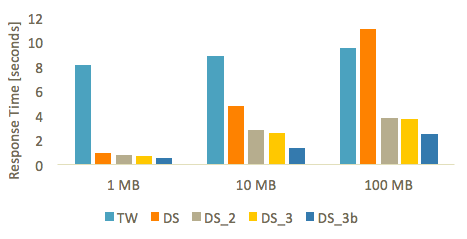
\includegraphics[scale=0.5]{images/exp1-load.png}
		\label{figure:load}
	}\hfill
	\subfigure[Sort Column]
	{
		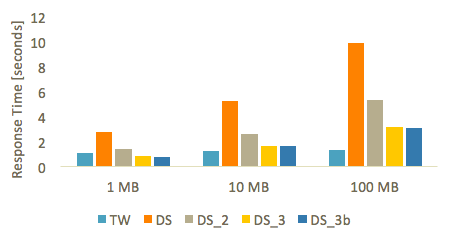
\includegraphics[scale=0.5]{images/exp1-sort.png}
		\label{figure:sort}
	}\hfill
	\subfigure[Drop Column]
	{
		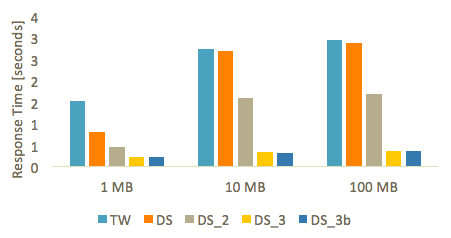
\includegraphics[scale=0.5]{images/exp1-drop.png}
		\label{figure:drop}
	}
	}
	\caption{Comparison of response times between DaSci and Trifacta Wrangler for three data operations.}
	\label{figure:exp1}
\end{figure} %figure*

\begin{figure}
	\centering
	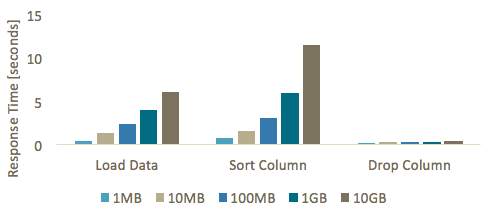
\includegraphics[scale=0.5]{images/exp1-all.png}
	\caption{DaSci's response time on binary data ($DS_{3b}$) with sampling, caching, and partitioning.}
	\label{figure:exp1-all}
\end{figure}


\subsection{Data Visualization}

We choose topic modeling as a use case to illustrate how DaSci can be used for data visualization.
Topic modeling aims at finding structure within an unstructured collection of documents by automatically inferring the underlying topics.
Inferred topics can then be used to summarize documents, further extract features, or map documents in low-dimensional space.

Figure \ref{figure:exp2} show the datagrid after and before applying the following transformations. We start data wrangling with a datagrid containing three columns, namely $abstract$, $links$ and $title$. In few minutes, we were able to
delete column $links$,
filter out NULL values in column $abstract$,
tokenize column $abstract$,
%convert $abstract$ back to string,
split column $title$ into $title1$ and $title2$ using character ":" ,
rename columns $title1$ and $title2$ as $source$ and $title$ respectively,
derive a label column $source\_label$ based on $source$, 
sort column $title$ in ascending order, and
derive five topics from column $abstract$ using LDA, creating one new column for each topic. 

Latent Dirichlet Allocation (LDA) is one of the most successful topic modeling techniques.
Initially developed for population genetics, LDA is now used as a reference for text analysis.
LDA is not given any topics and must instead infer them from raw text by defining a topic as a distribution over words.
Table \ref{table:lda} shows an example of topics inferred from Wikipedia's articles. In addition, LDA describes which topics each document is about. For instance, a document can be 40\% about "Topic 1" (politics) and 60\% about "Topic 2" (demography).

\begin{table}[H]
	\centering
	
  \begin{tabular}{llllll}
	\toprule
    \multicolumn{2}{l}{Topic 1} &
    \multicolumn{2}{l}{Topic 2} &
    \multicolumn{2}{l}{Topic 3} \\
    \midrule
    president & 0.03 & district & 0.06 & world & 0.04 \\
    state & 0.02 & village & 0.05 & gold & 0.04 \\
    member & 0.01 & populat. & 0.04 & champ. & 0.03 \\
    \bottomrule
  \end{tabular}
	
%	\begin{tabular}{lllllll}
%	\toprule
%	%\multicolumn{2}{c}{Name} \\
%	%\cmidrule(r){1-2}
%	$a$ & $b$ & $c$ & $d$ & $e$ & $f$ & $g$ \\
%	\midrule
%	$a_1$ & $b_1$ & $c_1$ & $null$ & $null$ & $null$ & $null$ \\
%	$a_2$ & $b_2$ & $c_2$ & $d_2$ &  $e_2$  & $null$ & $null$ \\
%	$null$ & $b_3$ & $c_3$ & $d_3$ &  $e_3$  & $null$ & $null$ \\
%	$null$ & $null$ & $null$ & $null$ &  $null$  & $f_4$ & $g_4$ \\
%	$null$ & $null$ & $null$ & $null$ &  $null$  & $f_5$ & $g_5$ \\
%	\bottomrule
%	\end{tabular}	
	
	
%  \begin{tabular}{|l|l|l|l|l|l|l|}
%    \hline
%    \multirow{2}{*}{Dataset} &
%      \multicolumn{2}{c}{A} &
%      \multicolumn{2}{c}{B} &
%      \multicolumn{2}{c|}{C} \\
%    & O.B.R & A.R & O.B.R & A.R & O.B.R & A.R \\
%    \hline
%    D1 & 2.1\% & 2.1\% & 2.1\% & 2.1\% & 2.1\% & 2.1\% \\
%    \hline
%    D2 & 11.6\% & 11.6\% & 11.6\% & 11.6\% & 11.6\% & 11.6\% \\
%    \hline
%    D3 & 5.5\% & 5.5\% & 5.5\% & 5.5\% & 5.5\% & 5.5\% \\
%    \hline
%  \end{tabular}

	\caption{Example of LDA topics learned from Wikipedia articles dataset  with their respective top-3 terms and weights \cite{lda}.}
	\label{table:lda}
\end{table}

We implement LDA on top of our data grid abstraction using Spark 2.0. First, we load the corpus of documents into DaSci and chose a vocabulary by pre-processing raw text contained in one of the columns. In our experiment, we perform the following preprocessing tasks: (i) we split raw text into terms following a bag-of-word approach, (ii) remove all non-alphabetic terms, (iii) remove short terms having less than three characters, (iii) exclude "stopwords", i.e. most common terms carrying little semantics, and (iv) perform term stemming to reduce inflected words into their root form.
Because the Spark ML module does not yet provide native support for natural language processing, DaSci uses NLTK to carry out stemming and stopword elimination.
%part-of-speech (POS) tagging to carry out stopword elimination and lemmatization.
 
We run LDA with five topics and 20 iterations over a subset of Wikipedia pages to obtain document distributions over topics. We use only five topics in order to get a concise summary of the document corpus, as comparing documents in a smaller feature space is more intuitive for users.
Another approach would be to run LDA using many topics and then to perform dimensional reduction and clustering. This is leaved as future work.
Next, we map the five topic vector into the column space and use the three most significant terms to name the derived columns.
Finally, we project documents in low-dimensional column space through a pivot chart.
In figure \ref{figure:exp2-topic1}, we use DaSci to visualize the derived topic \textit{"School Release Game"} as a bar chart over 100 Wikipedia pages.
Figure \ref{figure:exp2-topic2} shows the distribution of 1000 Wikipedia articles according to two topics, namely \textit{"Celtic Teenage Record"} and \textit{"Mythology Greek God"}.

\begin{figure*}[htp]
	\centering
	{
	\subfigure[Data before applying transformations.]
	{
		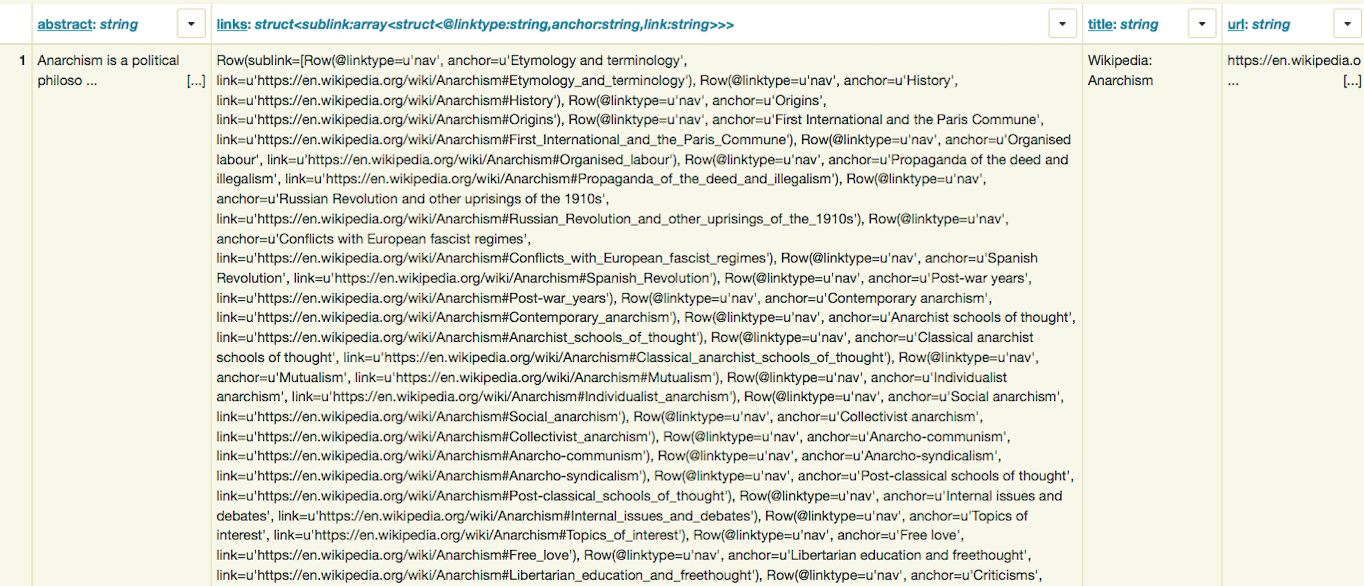
\includegraphics[scale=0.17]{images/exp2-grid1.png}
		\label{figure:exp2-grid1}
	}\hfill
	\subfigure[Data after applying transformations.]
	{
		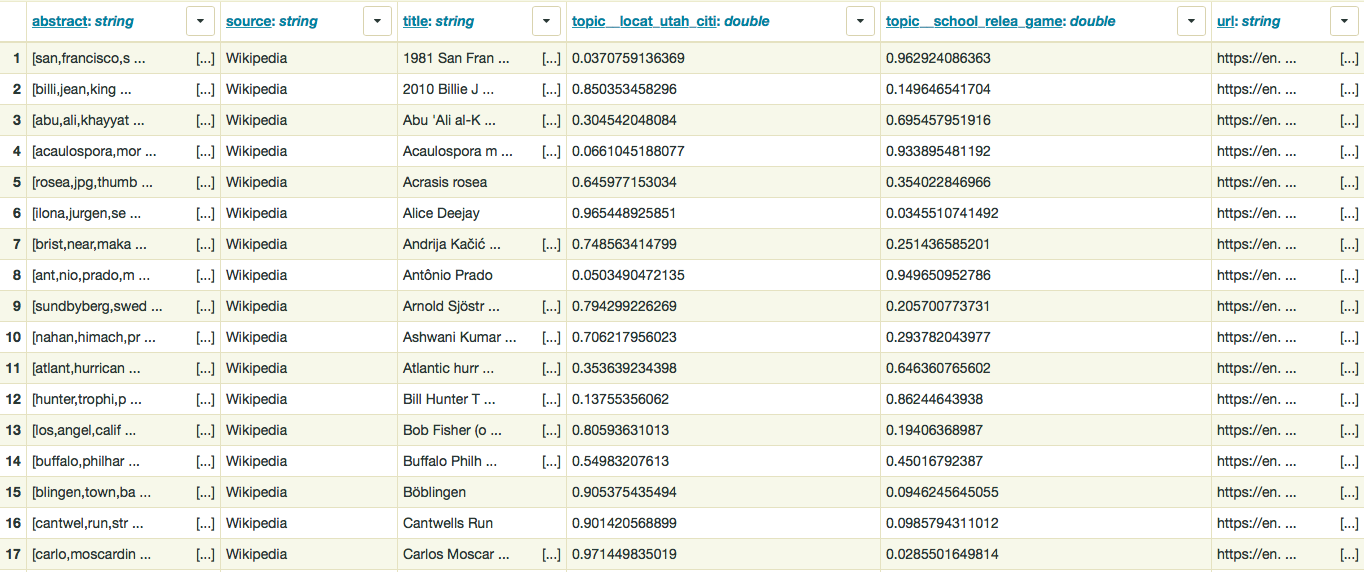
\includegraphics[scale=0.17]{images/exp2-grid2.png}
		\label{figure:exp2-grid2}
	}
	}
	\caption{Data Wrangling of Wikipedia Pages with DaSci.}
	\label{figure:exp2}
\end{figure*}

\begin{figure*}[htp] 
	\centering
	{
	\subfigure[Topic "School Release Game" for 100 pages.]
	{
		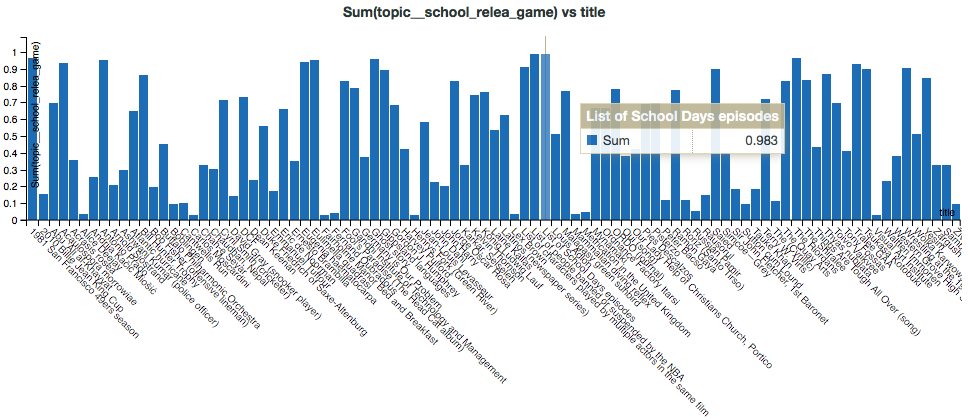
\includegraphics[scale=0.25]{images/exp2-topic1.png}
		\label{figure:exp2-topic1}
	}\hfill
	\subfigure[Topics "Celtic Teenage Record" vs. "Mythology Greek God" for 1000 pages.]
	{
		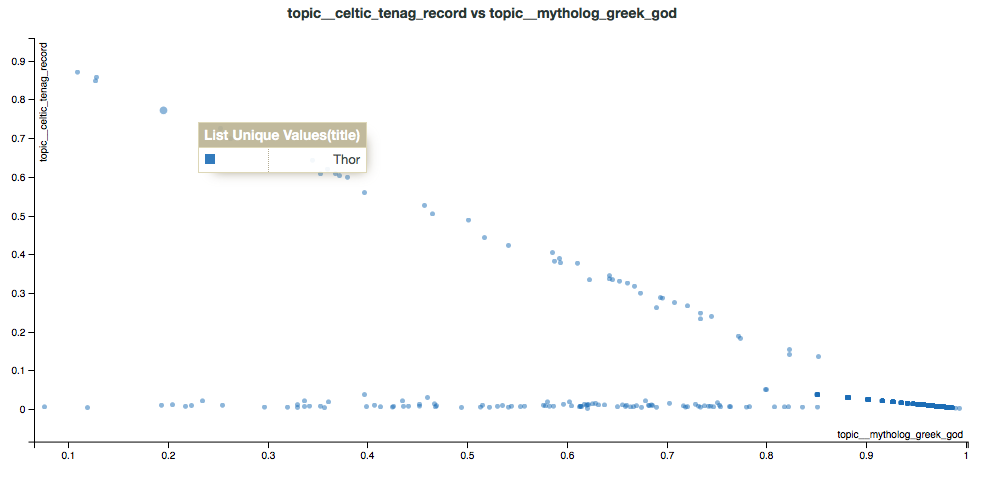
\includegraphics[scale=0.25]{images/exp2-topic2.png}
		\label{figure:exp2-topic2}
	}
	}
	\caption{Visualization of Wikipedia pages with DaSci.}
	\label{figure:exp2-view}
\end{figure*} 


%As final experiment, we measure the response time to derive topics using LDA. For this experiment, we reduce the number of iterations to one and increase the number of topics to 100. Results from 1 to 100 MB data size are shown in figure \ref{figure:exp2-lda-perf}.
%As we can see, performance are linear up until 10 MB, but deteriorate from 20 MB. This is due to a slow task that has very large size. 
%Similar experiments have been carried out by F. Liang et al. \cite{lda}.
%Their results illustrates the difference between the Online and Expectation-Maximization (EM) algorithms in Spark 1.5 by comparing the mean time per iterations, where iterations take 25.02 and 40.94 seconds respectively.
%
%\begin{figure}
%	\centering
%	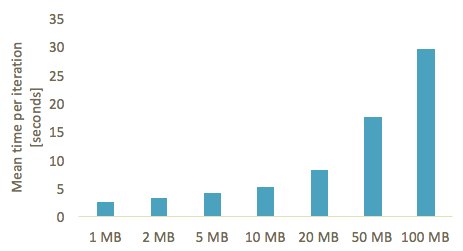
\includegraphics[scale=0.5]{images/exp2-lda-perf.png}
%	\caption{Training LDA with 100 topics on Wikipedia pages (mean time per iteration).}
%	\label{figure:exp2-lda-perf}
%\end{figure}


\subsection{Discussion}

All together, these experiments have confirmed our expectations by demonstrating clear performance improvements between the initial implementation and the more advanced infrastructure of DaSci. Experiments shows that our system can outperform in-production data-wrangling systems when sampling, caching and partitioning are enabled. 
Furthermore, we demonstrate that DaSci can successfully leverage machine learning capabilities in order to derive visual insights from textual data.

More experiments are naturally necessary to further validate that our system can cope with other data transformations. However, based on the current results, we are convinced that DaSci can already be used to perform data analysis over large, heterogeneous and potentially unstructured datasets.



\section{Future Work}
\label{section:future-work}

First of all, we plan to improve the \textit{u-join} algorithm.
Currently, \textit{u-join} is non-deterministic, as the algorithm can produces different results depending on the order in which datasets are joined.
For example, if datasets $R$, $S$, $T$ have schema $\{a,b\}$, $\{b,c\}$, and $\{c,d\}$ respectively, and each dataset contains a single record, then $R \Join_u S \Join_u T$ produces one tuple $\{a_1,b_1,c_1,d_1\}$, while $R \Join_u T \Join_u S$ produces two tuples $\{a_1,b_1,c_1,null\}$ and $\{null,b_1,c_1,d_1\}$.
We therefore plan to extend the \textit{u-join} to obtain deterministic behavior.
This is essential as we want the datagrid's column space to represent the underlying datasets as thoroughly as possible.

Now that we establish the foundation of DaSci, we intend to implement a whole set of new functionality to help data analysts getting insights about their unstructured datasets.
These new features include but are not limited to prefix/suffix elimination, aggregation functions (e.g. mode and median), and advanced machine learning algorithms such as clustering and classification (e.g. k-means and logistic regression, respectively).
From the machine learning perspective, we also plan to investigate how LDA could benefit from NLP techniques such as POS tagging and entity recognition, if these techniques were applied in earlier stages of the ML pipeline.

In the experiments presented in section \ref{section:experiments}, both server and cluster are deployed on the same machine.
Even though this is convenient to obtain a first assessment of our system, we need to conduct another round of experiments where servers and cluster are deployed on different machines. The idea is to investigate whether the current caching and sampling infrastructures can scale seamlessly according to the number of processing nodes.

Last but not least, a line of work that we plan to follow is to further investigate the canonical mapping between column space and vector space. Although more thorough inquiry is still needed, we are convinced that this is a promising approach that opens new perspectives for analyzing large unstructured datasets.

%------------------------------------------------

\section{Conclusion}
\label{section:conclusion}

In this work, we successfully design and implement DaSci, a system that allows large-scale textual data to be processed and visualized on the fly in real time.
In DaSci, the data is represented in a general-purpose, multi-dimensional datagrid that can be clustered, replicated, and retrieved efficiently.
Datagrid's dimensions can be assembled to form a large hypercube that can be further sliced, diced and aggregated though the pivot grid abstraction. 
DaSci combines the latest databases technologies together with machine learning algorithms used for textual information extraction, acting as a bridge between two multidimensional space, i.e. the vector space derived from raw text and the column space spanned by the OLAP hypercube.

We also demonstrate how data analysts and scientists can benefit from our novel infrastructure.
Complete control is given over the underlying datasets, such that analysts can define their own schema and taxonomy, as well as visualize trends in their datasets in a matter of seconds and without any IT expertise.
The experiments validate our approach, as our caching and sampling infrastructure drastically improves the response time compared to a more straightforward approach and, at the same time, outperforms in-production data-wrangling products. This first set of results is therefore convincing and a true motivation to undertake further work in this direction.


 
%------------------------------------------------

\section*{Acknowledgement}

I owe my deepest gratitude to Prof. Karl Aberer for allowing me to perform this work in the LSIR laboratory. I am also very thankful to Dr. Michele Catasta for his time and support, and for providing constructive and very much appreciated remarks during the realization of this work.

  
%----------------------------------------------------------------------------------------
%	REFERENCE LIST
%----------------------------------------------------------------------------------------

\begin{thebibliography}{99} % Bibliography - this is intentionally simple in this template

\bibitem{map-reduce} 
Jeffrey Dean and Sanjay Ghemawat. “MapReduce: simplified data processing on large clusters”. Google Inc. ACM 2008.

\bibitem{spark} 
Matei Zaharia, Mosharaf Chowdhury, Michael J. Franklin, Scott Shenker, and Ion Stoica. "Spark: Cluster Computing with Working Sets", University of California, Berkeley. HotCloud 2010.

\bibitem{spark-sql} 
M. Armbrust, R.S. Xin, C. Lian, Y. Huai, D. Liu, J.K. Bradley, X. Meng, T. Kaftan, M.J. Franklin, A. Ghodsi, M. Zaharia.
"Spark SQL: Relational Data Processing in Spark".
ACM 2015.

\bibitem{rdd} 
M. Zaharia, M. Chowdhury, T. Das, A. Dave, J. Ma, M. McCauley, M.J. Franklin, S. Shenker, I. Stoica. "Resilient Distributed Datasets: A Fault-Tolerant Abstraction for In-Memory Cluster Computing". USENIX 2012.

\bibitem{wrangler} 
S. Kandel, A. Paepcke, J. Hellerstein, and J. Heer. "Wrangler: interactive visual specification of data transformation scripts", Stanford University. SIGCHI 2011.

\bibitem{polaris} C. Stolte, D. Tang, P. Hanrahan. "Polaris: a system for query, analysis, and visualization of multidimensional relational databases"
IEEE 2002.

\bibitem{show-me} J. Mackinlay, P. Hanrahan, C. Stolte. "Show Me: Automatic Presentation for Visual Analysis". IEEE 2007.

\bibitem{seedb} A. Parameswaran, N. Polyzotis, H. Garcia-Molina. "SeeDB: visualizing database queries efficiently". ACM 2013.

\bibitem{nanocubes} L. Lins, J.T. Klosowski, C. Scheidegger. "Nanocubes for Real-Time Exploration of Spatiotemporal Datasets". IEEE 2013.

\bibitem{data-tiles} L. Battle, R. Chang; M. Stonebraker. "Dynamic Prefetching of Data Tiles for Interactive Visualization". SIGMOD 2016.

\bibitem{muck} 
Rebecca Weiss. "MUCK: A toolkit for extracting and visualizing semantic dimensions of large text collections". Stanford University. ACL 2014

\bibitem{mitext} 
Brendan O’Connor. "MITEXTEXPLORER: Linked brushing and mutual information for exploratory text data analysis". Carnegie Mellon University. ACL 2014.

\bibitem{core-nlp} C.D. Manning, M. Surdeanu, J. Bauer, J. Finkel, S.J. Bethard, D. McClosky. "The Stanford CoreNLP Natural Language Processing Toolkit". ACL 2014.

\bibitem{d3} M. Bostock, V. Ogievetsky and J. Heer. "$D^3$: Data-Driven Documents". IEEE 2011.

\bibitem{cell} G. Fourny. "Cell Stores". ETH Zurich, 28msec Inc, 2014.

\bibitem{etl} M. Castellanos, U. Dayal, S. Wang, G. Chetan. "Information Extraction, Real-Time Processing and DW2.0 in Operational Business Intelligence". Hewlett-Packard Laboratories, Palo Alto, CA, USA. 2010.

\bibitem{nltk-book}
Steven Bird, Ewan Klein, and Edward Loper, 
"Natural Language Processing with Python - Analyzing Text with the Natural Language Toolkit". O'Reilly.

\bibitem{nltk} NLTK: a platform for building Python programs to work with human language data. \\
http://www.nltk.org

\bibitem{trifacta} Trifacta Wrangler: fast and intuitive preparation of data on your desktop for analytic uses such as visualization. \\
https://www.trifacta.com/products/wrangler/

\bibitem{flask} Flask: a microframework for Python. \\
http://flask.pocoo.org

\bibitem{wikipedia} Wikipedia data dump downloads. \\
https://en.wikipedia.org/wiki/Wikipedia:\\Database\_download

\bibitem{lda} F. Liang, Y. Yang, J. Bradley. "Large Scale Topic Modeling: Improvements to LDA on Apache Spark.", Databricks Inc.

\end{thebibliography}

%----------------------------------------------------------------------------------------

%\end{multicols}

\end{document}
